\documentclass[10pt,twocolumn]{article}

\usepackage{algorithm}
%\usepackage{moreverb}   
%\usepackage{longtable}
\usepackage{fancyhdr}
\usepackage{algorithmic}             
%\usepackage{algorithm}
%\usepackage{array}     
\usepackage{hyperref}
\usepackage{graphicx}
\usepackage{subfigure}
\usepackage{fullpage}
\usepackage{amsmath, amssymb, amsthm}
%\usepackage[framed,numbered,autolinebreaks,useliterate]{mcode}
%\usepackage{mathabx}

% my macros
\newcommand{\paren}[1]{\left({#1}\right)}
\newcommand{\bracket}[1]{\left[{#1}\right]}
\newcommand{\curly}[1]{\left\{{#1}\right\}}
\newcommand{\vecb}[1]{\mathbf{#1}}
\newcommand{\matb}[1]{\mathbf{#1}}
\newcommand{\V}[1]{\mathbf{#1}}
\newcommand{\m}[1]{\mathbf{#1}}
\newcommand{\inhomog}[1]{\widetilde{#1}}
\newcommand{\transpose}[1]{{#1}^\top}

\usepackage{float}

\usepackage[margin=1in]{geometry}

\title{{\bf Intrusion Detection using Parzen-Windows on Provenance Graph Statistics}}
\author{
    Kenny Yu\\
    Harvard University\\
    \href{mailto:kennyyu@college.harvard.edu}{\texttt{kennyyu@college.harvard.edu}}
  \and
    R.J. Aquino\\
    Harvard University\\
    \href{mailto:rjaquino@college.harvard.edu}{\texttt{rjaquino@college.harvard.edu}}
}
\date{CS261, Fall 2013}

\begin{document}

\maketitle

%%%%%%%%%%%%%%%%%%%%%%%%%%%%%%%%%%%%%%%%%%%%%%%%%%%%
% ABSTRACT
%

\begin{abstract}
Security rests on being able to identify potentially malicious behavior.
One way to identify malicious behavior is to compare system behavior to known normal behavior.
Intrusions on a system typically leave behind digital artifacts, and we hypothesize
that we can detect intrusions on a system by identifying anomalies in the artifacts' {\em provenance}, or the lineage of how
the artifact came to be in its present state.
We present an intrusion detection approach to find these anomalies by analyzing provenance graphs statistics. We use a Parzen-Window approach \cite{parzen} on various provenance graph statistics \cite{clustering} 
to determine probability density estimates of normal behavior, and we use these density estimates to 
determine if an intrusion occurred. We used this approach to analyze simple intrusions on small provenance graphs and achieved promising results, however applying this technique to {\em user-to-remote} (u2r) intrusions 
from the much larger 1998 DARPA Intrusion Detection data sets  \cite{darpa} resulted in normal and abnormal behavior being indistinguishable. We discuss why we received the results we obtained for each of these workloads, and we propose requirements on intrusion detection models using provenance graph models that are necessary for the model to scale to large provenance graphs.

\end{abstract}

%%%%%%%%%%%%%%%%%%%%%%%%%%%%%%%%%%%%%%%%%%%%%%%%%%%%
% INTRODUCTION
%

\section{Introduction}

For as long as systems have existed, there have been malicious users that attempt to exploit vulnerabilities
in systems to gain unintended privileged access. As a result, system designers and 
administrators place a large effort in securing systems and preventing intrusions. However, intrusions
inevitably occur because of bugs or flaws within the system, and as a result, system administrators want to
have some automatic way of detecting these intrusions. 

Intrusions often leave behind digital artifacts, e.g., unusual output or log files, a process executed
with an unusual arguments or environment, unusual system call activity by a process. In addition to
unusual digital artifacts, we hypothesize that
intrusions also leave behind abnormalities
in the {\em provenance} of these digital artifacts, the lineage of how these digital artifacts were created.

Provenance is data that describes how digital artifacts
came to be in their current state. Provenance data is typically structured as a directed acyclic graph with
typed nodes and typed edges.
Nodes typically include processes and files, and edges are directed from nodes to their dependencies. For example,
process nodes have edges directed towards input file nodes and to the parent process's node, and
file nodes have edges directed towards previous versions of the file and to the nodes of the
processes that modified the file. See Figure 1 for an illustration of these provenance
graph node and edge types.

Existing intrusion detection systems (IDS) use provenance data only to a limited extent.
Allen et al. analyze
basic statistics on provenance graphs (e.g., number of nodes, number of edges, max number of edges per node, etc.) in order to facilitate
easier manual intrusion detection by a human \cite{provstat}. Their work, however, does not present a way of using provenance
graphs to automatically determine intrusions. Other systems use provenance data to determine the scope of an
intrusion. For example, Backtracker \cite{backtracker} uses provenance graphs to build causality graphs of intrusions: once the
system has
determined an intrusion has occurred, the system follows the causality graph backwards determine the original source of the attack, and 
then it follows the causality graph forwards to determine all the objects tainted by the attack. However, the authors 
do not present a way of using provenance data to automatically detect intrusions.

\begin{figure}
  \label{graph-simple}
  \centering
    \includegraphics[width=0.5\textwidth]{img/graph-simple.png}
    \caption{Example of a provenance graph, showing the types of nodes and edges common in provenance graphs} 
\end{figure}

In this paper, we present an approach to use provenance data to automatically detect intrusions. Intrusion
detection can be framed as a {\em novelty detection} problem, in which one attempts to decide whether
an unknown test pattern is produced by an underlying distribution corresponding to a training set
of normal patterns \cite{parzen}. However, Yeung et al. note that in the case of intrusion detection, novel
or abnormal patterns are typically difficult to obtain, and as a result, they present a {\em Parzen-Window} approach that allows them to characterize abnormal behavior by only knowing normal behavior.
Using this technique, they obtain a high degree of success
in identifying various intrusion types \cite{parzen}. Because obtaining abnormal patterns is difficult, 
we borrow their Parzen-Window approach to build models of normal behavior using 
various provenance graph statistics and graph centrality metrics, and we evaluate the success of this technique
on {\em user-to-local} (u2l) intrusions, intrusions that provide unauthorized access to local superuser (root) privileges.

The main contributions of this paper are the following:
\begin{enumerate}
\item Discuss which provenance graph statistics we chose to use, how we chose them, and why we chose them.
\item Analyze the Parzen-Window technique with various provenance graph statistics on a small data set and a real intrusion detection data set and evaluate its accuracy on both.
\item Discuss the limitations of the approach and propose requirements for provenance graph intrusion detection models to scale to larger-sized graphs.
\end{enumerate}


%%%%%%%%%%%%%%%%%%%%%%%%%%%%%%%%%%%%%%%%%%%%%%%%%%%%
% RELATED WORK
%

\section{Related Work}

\subsection{Existing IDSs using Provenance}

Many existing intrusion detection systems use provenance in some limited capacity; however, none of them
have used provenance for a fully automated detection system. 
Somayaji and Forrest's work in analyzing sequences of system calls for intrusion detection \cite{somayaji, somayaji-recent} can
be seen as one of the earliest works in building an intrusion detection system using provenance: sequences of
system calls can be seen as a limited form of provenance, as many systems build provenance graphs from
system call traces \cite{spade}. By analyzing the sequences
of system calls a process makes over time, their system builds a profile of ``normal" process behavior. When
the process in the future makes enough patterns of unrecognized sequences of system calls, the system flags
this process as behaving abnormally and attempts to stop the process, either through exponentially slowing down
system calls or aborting system calls entirely. Notably, their system is trained only by analyzing ``normal" data
without knowing explicitly what is considered ``abnormal." Because their system achieves high
accuracy in determining intrusions with only sequences of system calls, we believe that having real provenance
data in a graph structure--which in theory would be a superset of system call data--would allow us
to achieve comparable, if not better intrusion detection accuracy.

More recent work make use of the structure of provenance as a directed graph for a semi-automatic form
of intrusion detection, and to determine the scope of an intrusion. King et al. developed Backtracker \cite{backtracker}
 a modified
Linux kernel that tracks dependencies between operating system objects (files, processes, file names) similar
to provenance graphs. Backtracker builds a backwards causal graph to determine the entry point of an intrusion,
and it builds a forward causal graph to determine possibly tainted files, processes, or hosts in a distributed
system. However, Backtracker does not provide a way of automatically determining if an intrusion occurred
using provenance data; the provenance graph structure is only utilized after-the-fact.

Allen et al. make use of simple provenance graph statistics to categorize provenance graphs and to assist a human
in manual intrusion-detection \cite{provstat}. Given a data set of many provenance graphs, they calculated basic statistics
on the graphs (e.g., total nodes, total edges, max incoming edges on a node, max outgoing edges on a node,
node/edge ratio, average total edges per node, etc.). Their approach allows a human to more easily
notice anomalies in provenance graphs, but they do not provide a way to automate this detection.
We borrow their ideas of using simple provenance graph statistics as features to detect intrusions.

These works demonstrate that provenance data is indeed useful in collecting information about intrusions, and
Somayaji and King's work suggests that it might be possible to build a fully automated intrusion detection
system by making use of the graph structure of provenance.

\subsection{Parzen-Windows}

To address the difficulty of obtaining abnormal patterns for novelty detection on intrusion detection, we borrow
the Parzen-Window model approach proposed by Yeung et al.
They attempt to solve the lack of abnormal patterns problem by using Parzen-Windows to build {\em nonparametric}
density estimations of normal behavior \cite{parzen}. A density estimation is considered {\em nonparametric} if the estimation
makes no assumptions about the forms of the PDFs, except that PDFs are smooth. By using a nonparametric
density estimation, one can build a probability density estimate of normal behavior by only having examples of normal
behavior and no examples of abnormal behavior.

A {\em Parzen-window} estimate of a probability density function $p(\m{x})$
based on $n$ examples in a dataset $D$ drawn from model $\mathcal{M}$ is given by:
$$p(\m{x}) = \frac{1}{n} \sum_{i=1}^n \delta_n (\m{x} - \m{x_i})$$
where $\delta_n(\cdot)$ is a kernel function. They chose to use radially-symmetric Gaussian kernel functions because
Gaussian functions are smooth and therefore $p(\m{x})$ will be smooth, and because a radially-symmetric Gaussian function
can be specified by a single parameter, the variance of the kernel. Using a common variance $\sigma^2$ for all
the Gaussian kernels, we can rewrite $p(\m{x})$ as:
$$p(\m{x}) = \frac{1}{n(2\pi)^{d/2} \sigma^d} \sum_{i=1}^n  \exp \left\{  - \frac{|| \m{x} - \m{x_i}||^2}{2 \sigma^2}  \right\}$$
where $d$ is the dimensionality of the feature space $\m{x}$.

Let $\omega_1$ denote the state of being normal and $\omega_0$ the state of being abnormal.
To test if an example $\m{x} \in \omega_1$, they reframe the problem using hypothesis testing. Let $\m{y}$ be
an arbitrary example from $D$ drawn from $\mathcal{M}$, and let 
$$L(\m{y}) = \log p(\m{y})$$
be the log-likelihood of $\m{y}$ with respect to $\mathcal{M}$. Then we test the hypothesis that
$L(\m{x})$ is drawn from the distribution of the log-likelihood of the random examples in $D$ with:
\begin{eqnarray*}
P(L(\m{y}) \leq L(\m{x})) 
&=&  \frac{\#\m{y} \mbox { with } L(\m{y}) \leq L(\m{x})}{n} \\
&>& \psi
\end{eqnarray*}
for some threshold $0 < \psi < 1$, called the {\em false detection rate}. 
Thus, $\m{x} \in \omega_1$ is behaving normally if and only if $P(L(\m{y}) \leq L(\m{x})) > \psi$. 

In this paper, we use this same model to build profiles of ``normal" behavior for each process. We use
one-dimensional feature vectors $x$, and we use various provenance graph statistics and graph
centrality metrics as our features. We describe the various statistics and graph centrality metrics we explored
in the following section. For the common variance of our Gaussian kernels, we chose
the variance to be the variance of the data set $D_P$ for each unique process name $P$. 
We vary the features we used and values of $\psi$ and evaluate its performance on an intrusion detection data set.

\subsection{Provenance Graph Features}

We were inspired by the work proposed by Allen et al. who use simple provenance graph statistics to aide
in manual intrusion detection by humans. We extend their idea to make use of the typed node and typed edge
nature of provenance graphs \cite{provstat}. For example, instead of simply counting number of edges from a node, we
counted number of edges of type {\em input} directed towards {\em file} type nodes, or the number of {\em fork}
edges from {\em process} type nodes.

Furthermore, we hypothesize that intrusions manifest as anomalies in the lineage of digital artifacts, and
one way of observing this is through {\em graph centrality metrics}. A {\em graph centrality metric} is a function
of a node and its containing graph, and intuitively represents how {\em central} or {\em important} the node
is in the graph. In terms of provenance graphs, processes of the same program typically behave similarly to one another
and this should result in similar number of inputs, outputs, number of ancestors, and number of descendants for normal
process nodes of the same program.
Intrusions typically change the number of expected inputs and outputs (e.g., a process forking a shell process
when it normally does not), and we hypothesize that this can manifest as unusual changes in centrality
for the offending node in the provenance graph. Macko et al. note the following 3 observations unique to provenance graphs \cite{clustering}:
\begin{enumerate}
\item The ubiquity (importance) of a node is a function of a node's descendants, not its ancestors. (Note: Because edges in provenance graphs are in the direction of data dependence instead of data flow, ``descendants" in this case means ancestors in the provenance graph).
\item There is no agreed-upon granularity in which provenance should be captured.
\item Provenance has a temporal component.
\end{enumerate}

Using these observations, they propose several centrality metrics on provenance graphs:
\begin{itemize}
\item \textbf{In-degree Centrality}. Because a node's importance is based on its output descendants, then the number of times a node was used as input to another node indicates a simple measure of importance.
\item \textbf{Age}. They note that large "jumps" in timestamps or age might indicate breaks between tasks, but this interpretation is complicated when scripts execute tasks in short succession.
\item \textbf{Ancestor Centrality}. This measures the total number of descendants of a node, normalized by the total number of nodes in a graph.
\item \textbf{Opsahl's Closeness Centrality}. This accounts for the number of edges between a node and its descendants. To compute this, we calculate
$$CC'(v) = \sum_{x \in V -  \{v\}} (d'_{xv})^{-1}$$
where $V$ is the set of nodes in the graph, $d'_{xv}$ is the distance from node $x$ to $v$ by only following outgoing edges from $x$. Unreachable nodes from $x$ will have $d'_{xv} = \infty$, and so $(d'_{xv})^{-1} = 0$.
\item \textbf{Provenance Eigenvector Centrality}. The centrality of the nodes is given by the left dominant eigenvector of the matrix:
$$M_{ij} =
\begin{cases}
1 & \text{if there is an edge } i \to j \\
1/|V| & \text{if there is no out edge from } i \\
0 & \text{otherwise}
\end{cases}
$$
\end{itemize}
We implemented some of these graph centrality metrics and used Parzen-Windows on centrality measurements to compute density estimates for each process.

\subsection{Intrusion Types}

The DARPA Intrusion Detection Data Sets \cite{darpa} describe various kinds of intrusions in a network, including:
\begin{enumerate}
\item {\bf Denial of Service (dos)}. Intrusion that results in denial of service, e.g., overwhelming a server.
\item {\bf Remote to Local (r2l)}. Unauthorized access from a machine, e.g., guessing passwords.
\item {\bf User to Root (u2l)}. Unauthorized access to local superuser (root) privileges, e.g., various buffer overflow attacks.
\item {\bf Probing (probe)}. Surveillance and scanning, e.g. port scanning.
\end{enumerate}
Because we only collect provenance graphs local to the machine, we chose to limit our intrusion detection system only to u2l intrusions within this paper, as the other types of attacks involve exploiting the network and would not appear in provenance data.


%%%%%%%%%%%%%%%%%%%%%%%%%%%%%%%%%%%%%%%%%%%%%%%%%%%%
% DESIGN
%

\section{Design and Implementation}

We envision a provenance aware system which constantly builds normal profiles of processes. Simultaneously,
the system looks for instances of deviation from normal behavior and handles them appropriately
(e.g., terminating the process, slowing down the process). In our work, we derive normal profiles of process behavior
from provenance graphs, and we use a Parzen-Window model on various provenance graph statistics
to determine if anomalous nodes appear in the graph.

\subsection{Preliminary Provenance Exploration}

To determine which provenance statistics seem useful, we first created simple simulated intrusions
and ran them in a Provenance Aware Storage System (PASS) \cite{pass}, a file system with
a mounted volume that automatically collects provenance of all files within that volume.
To make data collection easier, we used PASSv2 \cite{passv2}, which provides an Ubuntu virtual machine with the PASS volume already installed.

For each of our intrusions, we ran it normally multiple times and collected the provenance. We then ran the
intrusion with the exploit multiple times and collected the new provenance.

We used the following procedure to implement our Parzen-Window density estimates and to decide whether a node is behaving normally or abnormally.
\begin{enumerate}
\item For each statistic that we implemented, we computed the counts for that statistic for all the
nodes in the provenance graph containing the normally-behaving workload.
\item We aggregated the counts by the name of the process (the path to the executable). For a given process name $P$, denote the
set of counts for that process name as $D_P$.
\item For each $y \in D_P$, calculate the log-likelihood $L_P(y)$.
\item For a test node with process name $P$ in the exploited-workload provenance graph, we calculate the value $x$ of the statistic in its graph, and then compute $L_P(x)$. 
If the ratio of the number of nodes $y$ with $L_P(y) \leq L_P(x)$,
to the total number of nodes in $D_P$ is greater than the false detection rate $\psi$, we label the node as normal. Otherwise we label the node as
an intrusion.
\end{enumerate}

In the exploited workloads, we used Orbiter \cite{orbiter} to find the abnormally behaving node by hand, and we used these nodes as our test nodes.

\subsection{Simulated Intrusions}

\subsubsection{hello}
We found that many of the popular exploits \cite{metasploit, exploitdb} involved buffer overflows and arbitrary code execution to possibly obtain root access. We used this as an guide to create a simple exploited \texttt{hello} program that echoes standard in to standard out, and we gave it a buffer overflow vulnerability that allows a malicious user to fork a shell.

We ran \texttt{hello} normally 40 times on various inputs and collected the provenance times. We then exploited the buffer overflow vulnerability in \texttt{hello} to spawn an \texttt{ls} process, and saved the standard out of that process to a file. See Figure 2 for examples of provenance graphs for the normally behaving and exploited versions of the program.

\subsubsection{mcrypt}
The mcrypt encryption package had a long standing buffer overflow, which would allow a malicious user to run their own code when mcrypt tried to decrypt the crafted exploit file. Due to limitations in our Virtual Machine set up, we were unable to exploit the vulnerable version of mcrypt, much like the authors of Backtracker \cite{backtracker} found. To emulate this exploit, we designed a Python program, which would decrypt (via ROT13) an input file. When sent a particular exploit file which contained malicious lines, our program would stop decrypting and start running the code specified in the file.

We ran our program on over 200 good inputs, and stored the provenance data. We then ran our program on two bad inputs, first to call \texttt{ls} as a Proof of Concept, and again to call \texttt{/bin/sh} to demonstrate that more severe attacks can be performed. We again exported the provenance generated from this exploited workload. See Figure 3 for examples of provenance graphs for the normally behaving and exploited versions of the program.

\begin{figure*}
  \label{hello-orbiter}
  \caption{Descendants of a \texttt{hello} program. The top image shows multiple invocations of a \texttt{hello} behaving normally when invoked with \texttt{cat foo.txt | ./hello > c.txt}. The bottom image shows \texttt{hello} being exploited to fork an \texttt{ls} process.} 
  \centering
    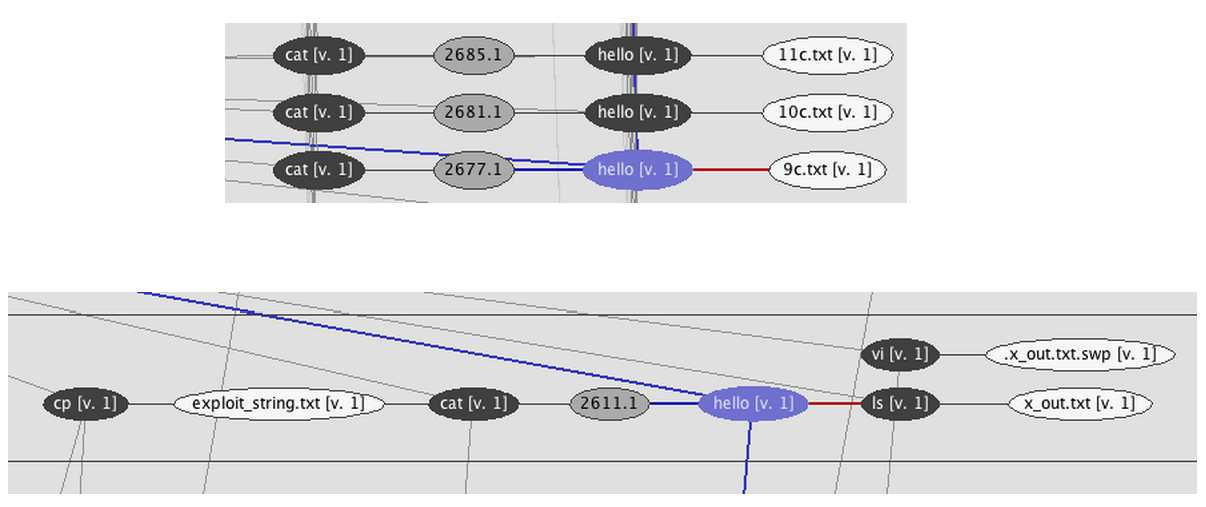
\includegraphics[width=\textwidth]{img/hello.png}
\end{figure*}
\begin{figure*}
  \label{mcrypt-orbiter}
  \caption{Descendants of an unexploited mcrypt-style program. Simply an output file. Below, descendants of an exploited mcrypt-style program. In addition to an (offscreen) output file, there is also an outgoing \texttt{/bin/sh} process, with its own children.}
  \centering
    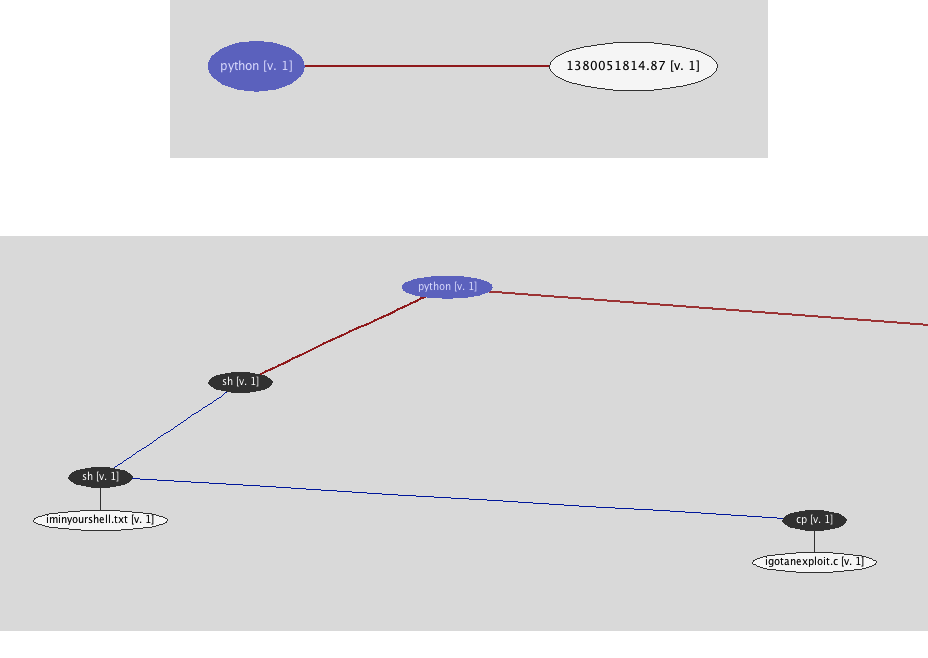
\includegraphics[width=\textwidth]{img/mcrypt.png}
\end{figure*}

\subsubsection{gcc}
Another type of exploit is more reminiscent of a system administration failure. By unexpectedly aliasing an important command, a user can unknowingly grant root access to a malicious program. To emulate this system administration attack, we replaced \texttt{/usr/bin/gcc} with our own version of gcc, which, in addition to compiling the user's code (via a call to gcc), logs that the user has made a request and copies the files the user had tried to compile. 

For our system administration attack, we compiled the PASS toolset using \texttt{gcc}, and exported the provenance from these runs. We then replaced \texttt{gcc} with our exploited version, compiled the toolset several times with different configurations, and exported the provenance again.

\subsection{Selecting Provenance Statistics}

\begin{figure*}
  \label{kde-example}
  \centering
    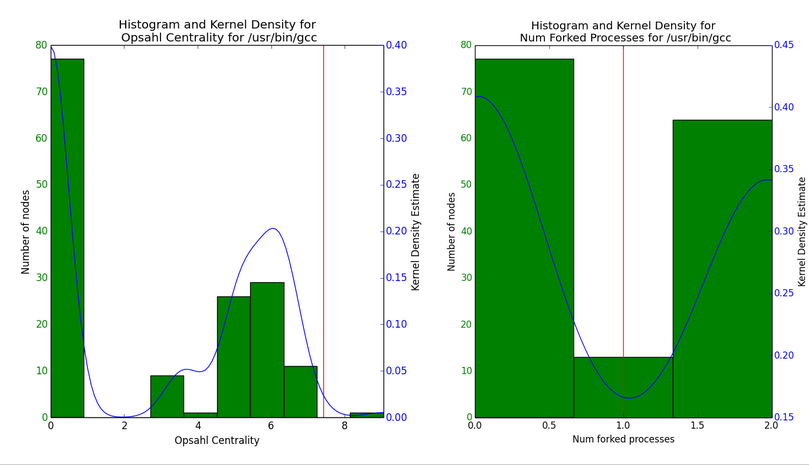
\includegraphics[width=\textwidth]{img/hist.png}
      \caption{Example Parzen-Window density estimates of a centrality measure and process statistic for the \texttt{gcc} exploit. The green bars represent the raw histogram counts, the blue curve represents the density estimate, and the red vertical line represents the estimation of a node of interest.}
\end{figure*}

\begin{table*}[ht]
\label{results}
{\small
  \begin{center}
  \begin{tabular}{| l | l | l | l |}
    \hline
    statistic & hello & mcrypt & gcc \\ \hline
     \# forked processes & 0.0 | 1 | 0.108 & 0.0 | 1 | 0.107 & 0.9 | 0 | 0.408 \\ \hline
     \# input files & 0.5 | 0 | 0.453 & 0.5 | 0 | 0.453 & 0.5 | 1 | 0.107 \\ \hline
     \# output files & 0.5 | 1 | 0.453 & 0.5 | 1 | 0.453 & 0.0 | 3 | 0.000 \\ \hline
    Opsahl centrality & 1.791 | 2.83 | 0.252 & 1.250 | 4.867 | 0.000 & 2.793 | 7.415 | 0.024 \\ \hline
    Ancestor centrality & 0.0009 | 0.0011 | 0.799 & 0.0002 | 0.0014 | 0.798 & 0.0007 | 0.0002 | 0.798 \\

    \hline
  \end{tabular}
  \end{center}
}
\hfill{}
\caption{average over good | test node value | density estimate of test node being ``normal"
}
\label{tb:tablename}
\end{table*}

Below is the list of simple provenance graph statistics we implemented:
\begin{enumerate}
\item number of input and output files
\item number of input and output processes
\item number of input and output pipes
\item number of versions stemming from this node
\end{enumerate}
We also implemented the indegree, Opsahl, and ancestor centrality metrics.
We chose not to implement the Provenance Eigenvector Centrality because computing
the eigenvectors of the large matrix took too much computation time on our machines.
We also chose not to implement age because age would make our data too dependent
on how quickly we executed our workloads.

In Table 1, we show a summary of the statistics that had any statistical difference between normal and abnormally behaving nodes, and Figure 4 highlights the most salient statistics for the \texttt{gcc} exploit. The buffer overflows showed the most abnormal behavior in the number of outgoing processes and the centrality measures. This makes sense, as arbitrary code execution will generate additional processes. Of the centrality metrics we implemented, the Opsahl Centrality metric did the best in distinguishing an exploited node from normally behaving nodes. Because the Opsahl Centrality metric accounts for the number of edges between a node and all of its descendants, this centrality metric is very sensitive to the addition of nodes. Exploits that have additional outputs (e.g. new processes and output files through a remote shell), thus generate a higher Opsahl centrality metric for the offending node. The more active the exploit is (say, if it forks a user shell), the more the centrality measure will be impacted, and the more likely it is that the exploit will be caught by our model.

If the exploit does not directly generate additional files, however, statistics like ``number of output files" will fail to be statistically significant. Indeed, the two programs (hello and mcrypt) that did not generate additional files were not flagged by that measure. On the other hand, the node representing the exploited version of \texttt{gcc} had abnormal density estimates, as it generated many more files than a normal \texttt{gcc} process. 

Because of this exploratory analysis, we chose to implement Opsahl centrality and analyze its accuracy on a real intrusion detection data set.

%%%%%%%%%%%%%%%%%%%%%%%%%%%%%%%%%%%%%%%%%%%%%%%%%%%%
% EVALUATION
%

\section{Evaluation}

\subsection{Experimental Setup}

We evaluated our approach by analyzing its accuracy on the 1998 DARPA Intrusion Detection Challenge data set \cite{darpa}.
The data set consists of users of several weeks of network-based attacks in the midst of normal
background data. The data includes BSM (Basic Security Model) traces \cite{bsm}, which provide an
audit of all the system calls made within a certain time period. The data also includes a list
of specific moments in time $T$ and the type of intrusion that occurred, if any.

For our experiments, we limited the scope of our intrusion detection system to only u2r attacks, as
the other kinds of attacks were network-based and would not appear in the provenance data. 
We identify each workload with a tuple:
$$(\psi, W)$$
where $\psi$ is our false detection rate for our Parzen-Window
estimates, and $W$ is the time window that we use to form time intervals to look for anomalous nodes. We used
the following procedure to evaluate the accuracy of our system: 
\begin{enumerate}
\item Use BSM traces to build provenance graphs, in a similar fashion to SPADE \cite{spade}. 
\item Compute the Opsahl centrality of the nodes in the graph and create a mapping from each process
name $P$ to a list of log-likelihood values $L(y)$, where $y$ is the computer centrality measurement for each node in the graph having process name $P$.
\item For a specific moment in time $T$, find all edges in the provenance graph we built with timestamps in the interval $[T - W, T + W]$. 
Use the nodes attached to these edges as our {\em candidate anomaly set}. We used the specific times listed in data sets for our values of $T$.
\item For all nodes in the candidate anomaly set, find the process name $P$ of the node, and use our Parzen-Window approach on process
name $P$ to determine if the node is anomalous. We evaluate whether a node is normal or anomalous using the Parzen-Windows built from the graph
containing the node.
\item For times $T$ in the data set listed as having an intrusion, our intrusion detection system considers that time $T$ as having an intrusion
if a {\em majority} of the nodes in the candidate anomaly set are considered anomalous.
\end{enumerate}

For each $(\psi, W)$, we compute:
\begin{itemize}
\item {\em False Positive Rate (FPR).} Ratio of number of time intervals that do not actually contain an intrusion
but were misidentified as having an intrusion, to the total number of time intervals.
\item {\em True Positive Rate (TPR).} Ratio of the number of time intervals that actually do contain an intrusion
and were correctly identified as having an intrusion, to the total number of time intervals.
\end{itemize}

We evaluated the accuracy of our system on various values of $\psi$ and $W = 10s, 100s, 1000s$.

\subsection{Results}

\noindent
\begin{figure}
  \label{tpr}
  \centering
    \includegraphics[width=0.5\textwidth]{img/tpr.png}
    \caption{True Positive Rate. The window size 10s, 100s, 1000s did not impact the true positive rate at all for various values of $\psi$.} 
\end{figure}

\noindent
\begin{figure}
  \label{fpr}
  \centering
    \includegraphics[width=0.5\textwidth]{img/fpr.png}
    \caption{False Positive Rate. The window size 10s, 100s, 1000s did not impact the false positive rate very
    much for various values of $\psi$.} 
\end{figure}

We plot the true positive rates for various values of $\psi$ and window sizes $W$ in Figure 5, and similarly for the false positive rates in Figure 6.

We note that the true positive rate and false positive rates are nearly identical as we vary $\psi$. Furthermore, the true positive rate stayed exactly the same as we varied our window size $W$ from $10s, 100s, 1000s$. Thus, the window size had little to no impact on the TPR and FPR. As we increase $\psi$, the false detection rate, we expect to see more positives, and this is exactly what we see in these graphs.

\subsection{Discussion}

We note that the true positive rates and false positive rates were not what we expected. We were surprised to see that the true positive rates and false positive rates were nearly identical to each other. The fact that the TPR and FPR were identical to each other suggests that our Parzen-Window model using Opsahl centrality could not reliably distinguish between normal and abnormal behavior in the large graphs generated from the DARPA data set. 

We believe that the reason we had more promising results on our simulated intrusion data sets from PASS was because the provenance graphs from these workloads were much smaller (on the order of 5000 nodes). As a result of the much smaller size, small changes in provenance graph structure from an intrusion has a much profounder impact on the smaller provenance graphs. Thus, intrusions on our PASS workload had a much higher impact on the centrality calculations and resulted in more anomalous behavior in our Parzen-Window model. In the DARPA data set, we faced much larger provenance graphs (on the other of 20,000 nodes), and because of the much larger size, the effect of small changes in provenance graph structure from an intrusion had a much smaller impact on the overall structure of the graph. Intrusions did not change the centrality metrics very much in large graphs; therefore anomalous behavior went undetected, regardless of the window size we chose. Since our system could not distinguish between anomalous and normal behavior, then the true positive rate and false positive rate are essentially identical. From these results, we propose the following requirements for intrusion detection models that use provenance graph statistics in order to be useful for large provenance graphs:

\begin{itemize}
\item The effects of the provenance graph statistic should grow as the size of the provenance graph grows. Since provenance graphs are meant to be long-lived, a small anomaly in the provenance graph will be drowned out by the overall large structure of the graph. Thus, if a statistic only captures a small local property of the graph, that property will become negligible and the anomaly will go undetected. As a result, a provenance statistic should become {\em more} anomalous as more provenance is collected.

\item The statistic must be adaptive and computable online. In order to make a truly useful online intrusion detection system, the statistic must be recomputed quickly over all the nodes in the graph as the provenance graph grows. Possible examples of such a statistic could be progressive forms of PageRank where the rank is computed relative to a starting node.

\item The model must be able to predict anomalous behavior by being trained with only examples of normal behavior. As stated by Yeung et al., intrusion detection is a form of novelty detection where access to abnormal patterns is very difficult \cite{parzen}. As a result, successful intrusion detection models like Somayaji and Forrest's model must be able to characterize abnormal behavior without knowing precisely what that means.
\end{itemize}


%%%%%%%%%%%%%%%%%%%%%%%%%%%%%%%%%%%%%%%%%%%%%%%%%%%%
% CONCLUSION
%

\section{Future Work}

\subsection{N-distance Statistics}
Some processes fork helper processes that do the real work (such as \texttt{gcc}). We found that \texttt{gcc} forks processes for the linker/assembler that handles generating output, so \texttt{gcc} does not directly have output files. Similarly, when running a python script, the code file itself is not directly executed, it is read in by a python process, which then goes off and collects input, generates output, and forks additional processes. Thus, when running a python file, the file itself only has one node in the provenance graph, with many python process nodes accessing it. In order to account for these kinds of relationships, we could calculate the relevant statistics for the test node and all nodes at distance $N$ from the test node, and then aggregate them. By utilizing information about neighboring nodes, we hope to detect intrusions that involve more complicated relationships
between nodes.
\subsection{ENV and ARGV}
Currently we ignore the environment and argument information stored in the provenance graph. By generating histograms based on this information, we could catch subtler intrusions that rely on modified environment information. Additionally, if an exploit relies on a particular argument or argument patterns, this information might reflected in the ARGV information.
\subsection{Different values for the density variance}
In our system, we used the variance $D$ of each data set as the variance of our kernel. To possibly get better results, one might try using different values for the variance, possible values that capture more granularity of students.
\subsection{Online Intrusion Detection}
Currently, this system runs after-the-fact, but truly useful intrusion detection systems need to run while the system is online. To do this, we would need to modify our statistics to use centrality metrics that are {\em progressive}, i.e., they can be recomputed online without needing to recompute the metric on the entire graph. 

Given progressive forms of these statistics, we can modify PASS to compute Parzen-Window density estimates as it generates provenance, or we can audit system calls like SPADE \cite{spade} to build provenance graphs in user space and apply our Parzen-Window technique.
\subsection{Local vs. Global}
In our experiments, we looked at provenance graphs in their entirety. However, provenance graphs are meant to be long-lived, and an intrusion that affected only a small portion of the graph will have negligible effects on the global structure of the graph. To resolve this issue, a possible future extension to our work is to cluster the nodes based on time \cite{clustering} and then only examine the most ``recent" nodes when applying our histogram technique. Another approach would be to discard provenance data in computing Parzen-Window density estimates after the data have reached a certain age. By allowing the model to evolve over time, the system
can combat {\em autoimmune disorders} in which attackers purposely invoke programs in weird ways to fool the system into thinking the programs are
behaving abnormally.

\section{Conclusion}

In this paper, we frame the intrusion detection problem as a novelty detection problem, and we propose a model to use Parzen-Window estimates on provenance graph statistics to detect intrusions. Our model showed some success on small provenance graphs, but did not perform well on much larger provenance graphs. We discuss why we obtained these results, and we use these lessons to propose requirements for intrusion detection models that use provenance graphs.

%%%%%%%%%%%%%%%%%%%%%%%%%%%%%%%%%%%%%%%%%%%%%%%%%%%%
% ACKNOWLEDGEMENTS
%

\section{Acknowledgements}
We want to thank Margo Seltzer and Daniel Margo for their guidance on the direction of the project, for their help in working with PASS, and for their insight in analyzing provenance graphs. We also want to thank the members of the CS261 Program Committee for their feedback on the initial draft of this paper.


%%%%%%%%%%%%%%%%%%%%%%%%%%%%%%%%%%%%%%%%%%%%%%%%%%%%
% BIBLIOGRAPHY
%

\begin{thebibliography}{99}

\bibitem{provstat}
\textsc{Allen, D. M., Chapman, A., Seligman, L., and Blaustein, B.} Provenance for Collaboration: Detecting Suspicious Behaviors and Assessing Trust in Information. In {\em Proceedings of the International Conference on Collaborative Computing: Networking, Applications and Worksharing} (October 2011).

\bibitem{darpa}
\textsc{DARPA Intrusion Detection Evaluation Data Set, 1998.} {\tt http://www.ll.mit.edu/mission/\\communications/cyber/CSTcorpora/ideval/\\data/1998data.html}.

\bibitem{spade}
\textsc{Gehani, A. and Tariq, D.} SPADE: Support for Provenance Auditing in Distributed Environments. In {\em Proceedings of the 2012 ACM/IFIP/USENIX International Middleware Conference} (December 2012).

\bibitem{somayaji-recent}
\textsc{Inoue, H. and Somayaji, A.} Lookahead Pairs and Full Sequences: A Tale of Two Anomaly Detection Methods. In {\em 2nd Annual Symposium on Information Assurance} (June 2007). 

\bibitem{backtracker}
\textsc{King, S. T. and Chen, P. M.} Backtracking Intrusions. In {\em SOSP'03 Proceedings of the nineteenth ACM symposium on Operating systems principles} (December 2003).

\bibitem{clustering}
\textsc{Macko, P., Margo, D., Seltzer, M.} Local Clustering in Provenance Graphs (Extended Version). In {\em Proceedings of the 22nd ACM international conference on Conference on information \& knowledge management} (August 2013).

\bibitem{orbiter}
\textsc{Macko, P. and Seltzer, M.} Provenance Map Orbiter: Interactive Exploration of Large Provenance Graphs. In {\em TaPP'11 Proceedings of the 2nd conference on Theory and practice of provenance} (June 2011).

\bibitem{passv2}
\textsc{Muniswamy-Reddy, K., Braun, U., Holland, D. A., Macko, P., Maclean, D., Margo, D., Seltzer, M., and Smogor, R.} Layering in Provenance Systems. In {\em Proceedings of the 2009 USENIX Annual Technical Conference} (June 2009).

\bibitem{pass}
\textsc{Muniswamy-Reddy, K., Holland, D. A., Braun, U., and Seltzer, M.} Provenance-Aware Storage Systems. In {\em Proceedings of the 2006 USENIX Annual Technical Conference} (June 2006).

\bibitem{exploitdb}
\textsc{Offensive Security, Inc.} The Exploit Database. {\tt http://www.exploit-db.com}.

\bibitem{metasploit}
\textsc{Rapid 7 Inc.} Metasploit Framework. {\tt http://www.metasploit.com}.

\bibitem{somayaji}
\textsc{Somayaji, A. and Forrest, S.} Automated Response Using System-Call Delays. In {\em Proceedings of the 2000 USENIX Annual Technical Conference} (August 2000).

\bibitem{bsm}
\textsc{SunSHIELD Basic Security Module Guide.} {\tt http://docs.oracle.com/cd/\\E19455-01/806-1789/6jb25l4bc/index.html}.

\bibitem{parzen}
\textsc{Yeung, D. and Chow, C.} Parzen-Window Network Intrusion Detectors. In {\em Proceedings of 2002 International Conference on Pattern Recognition} (August 2002).

\end{thebibliography}

\end{document}
